%
% Capítulo 3
%
\chapter{Solução Proposta} \label{cap3}

Neste capítulo pretende-se dar ênfase à solução implementada para resolver o problema apresentado no capítulo \ref{cap2}. Este capítulo está divido nas seguintes secções, Modelo de Dados na secção \ref{sec31}, \acrlong{bd} na secção \ref{sec32}, Acesso a Dados na secção \ref{sec33} e Lógica de Negócio na secção \ref{sec34}.

\begin{figure}[H]
	\centering
	\includegraphics[width=12cm, scale=1]{./figures/project_structures.png}
	\caption{Estrutura do Projeto}
	\label{project-structure}
\end{figure}

\begin{center}
	\includegraphics[width=12cm, scale=1]{./figures/project_structures_caption.png}
\end{center}

Com a Figura \ref{project-structure} pretende-se não só apresentar os principais componentes do projeto, bem como demonstrar de forma breve a relação dos mesmos. É de destacar que uma \textit{tag} pode ser lida por um dispositivo de \textit{hardware} munido de um leitor de \textit{tags}. Um \textit{smartphone} equipado com tecnologia \acrshort{nfc} pode escrever na \textit{tag} \acrshort{nfc}, tal é necessário para identificar produtos avulsos presentes num sistema de arrumação. Tanto o dispositivo de \textit{hardware} como as aplicações, móvel e \textit{web}, comunicam com a \gls{api-web}.\\

O projeto é composto por 2 blocos principais, que se relacionam. A Figura \ref{project-architecture} representa esses blocos. 

\begin{figure}[H]
	\centering
	\includegraphics[height=9cm, scale=1]{./figures/project_architecture.png}
	\caption{Arquitetura do Projeto}
	\label{project-architecture}
\end{figure}

O lado do servidor incluí quatro camadas e expõe uma \gls{api-web}. A camada da \acrfull{bd} é realizada com o \acrfull{sgbd} \textit{PostgreSQL}. A \acrfull{dal} é responsável pelas leituras e escritas à \acrshort{bd}. Esta camada é produzida com a linguagem de programação \textit{Java}, com a \acrfull{jpa}. A \acrfull{bll} é responsável pela gestão dos dados obtidos da \acrshort{bd} ou dos \textit{controllers}. A implementação desta camada recorreu à mesma ferramenta que foi usada na \acrshort{dal}. Os \textit{controllers} foram desenvolvidos em \textit{Java} com a \textit{framework} da \textit{Spring}, chamada de \textit{Spring Boot}. A \gls{api-web} disponibiliza recursos em diferentes \textit{hypermedia}.

Do lado do cliente existem dois modos de interação, por uma aplicação móvel e outra por uma aplicação web. A aplicação móvel disponível para a plataforma \textit{Android}, desenvolvida em linguagem \textit{Kotlin}. A aplicação web é disponibilizada para a maioria dos browsers, implementada utilizando a linguagem \textit{JavaScript}, com o auxilio da \textit{framework Express}.

%
% Modelo de Dados
%
\section{Modelo de Dados}\label{sec35}






% Modelo EA
\subsection{Modelo Entidade-Associação}\label{subsec311}

\begin{figure}[H]
	\hspace*{-2,5cm}
	\centering
	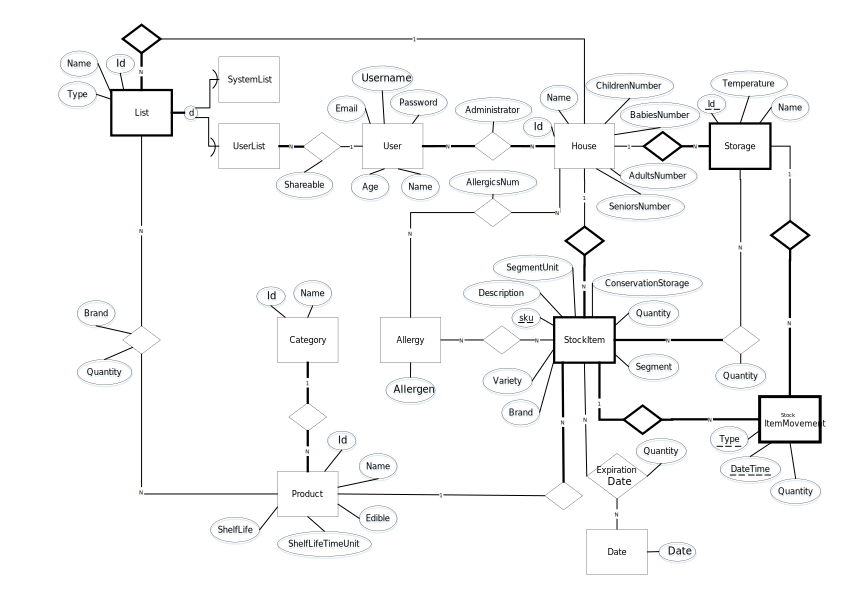
\includegraphics[width=20cm,height=15cm,scale=1]{./files/EA.pdf}
	\caption{Modelo Entidade-Associação}
	\label{modelo-ea}
\end{figure}

% Domínio dos Atributos
\subsection{Domínio dos Atributos}\label{subsec313}
\raggedbottom
% House
\begin{table} [H]
	\centering
	\caption{Domínio dos Atributos da Entidade House.} \vspace{2mm}
	\label{tab-dominio-atributos-house}
	\resizebox{\textwidth}{!}{%
		\begin{tabular}{|c|c|C{2.5cm}|C{2.7cm}|C{3.6cm}|C{2.3cm}|}
			\hline
			\textbf{Entidade} & \textbf{Atributo} & \textbf{Domínio} & \textbf{Tipo Variável (PostgreSQL)} & \textbf{Restrições} & \textbf{Nullable}\\ \hline
			\multirow{6}{*}{House} & house\_id & Número inteiro auto-incrementado & bigserial & - & não\\ \cline{2-6}
			& house\_name & Cadeia de caracteres de comprimento variável & character varying(35) & até 35 caracteres & não\\ \cline{2-6}
			& house\_characteristics & Objeto \acrshort{json} & json & - & não\\ \hline
		\end{tabular}
	}
\end{table}

% User
\begin{table} [H]
	\centering
	\caption{Domínio dos Atributos da Entidade User.} \vspace{2mm}
	\label{tab-dominio-atributos-user}
	\resizebox{\textwidth}{!}{%
		\begin{tabular}{|c|c|C{2.5cm}|C{2.7cm}|C{3.6cm}|C{2.3cm}|}
			\hline
			\textbf{Entidade} & \textbf{Atributo} & \textbf{Domínio} & \textbf{Tipo Variável (PostgreSQL)} & \textbf{Restrições} & \textbf{Nullable}\\ \hline
			\multirow{5}{*}{User} & user\_username & Cadeia de caracteres de comprimento variável & character varying(30) & até 30 caracteres & não\\ \cline{2-6}
			& user\_email & Cadeia de caracteres de comprimento variável & character varying(254) & até 254 caracteres & não\\ \cline{2-6}
			& user\_age & Número inteiro & smallint & user\_age in [0, 150] & não\\ \cline{2-6}
			& user\_name & Cadeia de caracteres de comprimento variável & character varying(70) & até 70 caracteres & não\\ \cline{2-6}
			& user\_password & Cadeia de caracteres de comprimento variável & character varying(50) & até 50 caracteres & não\\ \hline
		\end{tabular}
	}
\end{table}

% Allergy
\begin{table} [H]
	\centering
	\caption{Domínio dos Atributos da Entidade Allergy.} \vspace{2mm}
	\label{tab-dominio-atributos-allergy}
	\resizebox{\textwidth}{!}{%
		\begin{tabular}{|c|c|C{2.5cm}|C{2.7cm}|C{3.6cm}|C{2.3cm}|}
			\hline
			\textbf{Entidade} & \textbf{Atributo} & \textbf{Domínio} & \textbf{Tipo Variável (PostgreSQL)} & \textbf{Restrições} & \textbf{Nullable}\\ \hline
			{Allergy} & allergy\_allergen & Cadeia de caracteres de comprimento variável & character varying(75) & até 75 caracteres & não\\ \hline
		\end{tabular}
	}
\end{table}


% Recipe
\begin{table} [H]
	\centering
	\caption{Domínio dos Atributos da Entidade Recipe.} \vspace{2mm}
	\label{tab-dominio-atributos-recipe}
	\resizebox{\textwidth}{!}{%
		\begin{tabular}{|c|c|C{2.5cm}|C{2.7cm}|C{3.6cm}|C{2.3cm}|}
			\hline
			\textbf{Entidade} & \textbf{Atributo} & \textbf{Domínio} & \textbf{Tipo Variável (PostgreSQL)} & \textbf{Restrições} & \textbf{Nullable}\\ \hline
			\multirow{9}{*}{Recipe} & recipe\_id & Número inteiro auto-incrementado & bigserial & - & não\\ \cline{2-6}
			& recipe\_name & Cadeia de caracteres de comprimento variável & character varying(35) & até 35 caracteres & não\\ \cline{2-6}
			& recipe\_instructions & Cadeia de caracteres de comprimento variável & text & - & não\\ \cline{2-6}
			& recipe\_difficulty & Cadeia de caracteres de comprimento variável & character varying(9) & recipe\_difficulty in ['easy', 'average', 'difficult'] & sim\\ \cline{2-6}
			& recipe\_time & Número inteiro & smallint & recipe\_time \textgreater{} 0 & sim\\ \cline{2-6}
			& recipe\_servings & Número inteiro & smallint & recipe\_servings \textgreater{} 0 & sim\\ \cline{2-6}
			& recipe\_cuisine & Cadeia de caracteres de comprimento variável & character varying(35) & até 35 caracteres & sim\\ \cline{2-6}
			& recipe\_dishType & Cadeia de caracteres de comprimento variável & character varying(35) & até 35 caracteres & sim\\ \cline{2-6}
			& recipe\_type & Cadeia de caracteres de comprimento variável & character varying(7) & recipe\_type  in ['system', 'user'] & não\\ \hline
		\end{tabular}
	}
\end{table}

% System Recipe
\begin{table} [H]
	\centering
	\caption{Domínio dos Atributos da Entidade SystemRecipe.} \vspace{2mm}
	\label{tab-dominio-atributos-systemRecipe}
	\resizebox{\textwidth}{!}{%
		\begin{tabular}{|c|c|C{2.5cm}|C{2.7cm}|C{3.6cm}|C{2.3cm}|}
			\hline
			\textbf{Entidade} & \textbf{Atributo} & \textbf{Domínio} & \textbf{Tipo Variável (PostgreSQL)} & \textbf{Restrições} & \textbf{Nullable}\\ \hline
			{System Recipe} & recipe\_id & Número inteiro & bigint & recipe\_id \textgreater{} 0 & não\\ \hline
		\end{tabular}
	}
\end{table}

% User Recipe
\begin{table} [H]
	\centering
	\caption{Domínio dos Atributos da Entidade UserRecipe.} \vspace{2mm}
	\label{tab-dominio-atributos-userRecipe}
	\resizebox{\textwidth}{!}{%
		\begin{tabular}{|c|c|C{2.5cm}|C{2.7cm}|C{3.6cm}|C{2.3cm}|}
			\hline
			\textbf{Entidade} & \textbf{Atributo} & \textbf{Domínio} & \textbf{Tipo Variável (PostgreSQL)} & \textbf{Restrições} & \textbf{Nullable}\\ \hline
			\multirow{2}{*}{User Recipe} & recipe\_id & Número inteiro & bigint & recipe\_id \textgreater{} 0 & não\\ \cline{2-6}
			& user\_username & Cadeia de caracteres de comprimento variável & character varying(30) & até 30 caracteres & não\\ \hline
		\end{tabular}
	}
\end{table}

% Shared Recipe
\begin{table} [H]
	\centering
	\caption{Domínio dos Atributos da Entidade SharedRecipe.} \vspace{2mm}
	\label{tab-dominio-atributos-sharedRecipe}
	\resizebox{\textwidth}{!}{%
		\begin{tabular}{|c|c|C{2.5cm}|C{2.7cm}|C{3.6cm}|C{2.3cm}|}
			\hline
			\textbf{Entidade} & \textbf{Atributo} & \textbf{Domínio} & \textbf{Tipo Variável (PostgreSQL)} & \textbf{Restrições} & \textbf{Nullable}\\ \hline
			\multirow{2}{*}{Shared Recipe} & recipe\_id & Número inteiro & bigint & recipe\_id \textgreater{} 0 & não\\ \cline{2-6}
			& user\_username & Cadeia de caracteres de comprimento variável & character varying(30) & até 30 caracteres & não\\ \hline
		\end{tabular}
	}
\end{table}

% List
\begin{table} [H]
	\centering
	\caption{Domínio dos Atributos da Entidade List.} \vspace{2mm}
	\label{tab-dominio-atributos-list}
	\resizebox{\textwidth}{!}{%
		\begin{tabular}{|c|c|C{2.5cm}|C{2.7cm}|C{3.6cm}|C{2.3cm}|}
			\hline
			\textbf{Entidade} & \textbf{Atributo} & \textbf{Domínio} & \textbf{Tipo Variável (PostgreSQL)} & \textbf{Restrições} & \textbf{Nullable}\\ \hline
			\multirow{4}{*}{List} & house\_id & Número inteiro & bigint & house\_id \textgreater{} 0 & não\\ \cline{2-6}
			& list\_id & Número inteiro auto-incrementado & smallint & - & não\\ \cline{2-6}
			& list\_name & Cadeia de caracteres de comprimento variável & character varying(35) & até 35 caracteres & não\\ \cline{2-6}
			& list\_type & Cadeia de caracteres de comprimento variável & character varying(7) & list\_type  in ['system', 'user'] & não\\ \hline
		\end{tabular}
	}
\end{table}

% System List
\begin{table} [H]
	\centering
	\caption{Domínio dos Atributos da Entidade SystemList.} \vspace{2mm}
	\label{tab-dominio-atributos-systemList}
	\resizebox{\textwidth}{!}{%
		\begin{tabular}{|c|c|C{2.5cm}|C{2.7cm}|C{3.6cm}|C{2.3cm}|}
			\hline
			\textbf{Entidade} & \textbf{Atributo} & \textbf{Domínio} & \textbf{Tipo Variável (PostgreSQL)} & \textbf{Restrições} & \textbf{Nullable}\\ \hline
			\multirow{2}{*}{System List} & house\_id & Número inteiro & bigint & house\_id \textgreater{} 0 & não\\ \cline{2-6}
			& list\_id & Número inteiro & smallint & list\_id \textgreater{} 0 & não\\ \hline
		\end{tabular}
	}
\end{table}

% User List
\begin{table} [H]
	\centering
	\caption{Domínio dos Atributos da Entidade UserList.} \vspace{2mm}
	\label{tab-dominio-atributos-userList}
	\resizebox{\textwidth}{!}{%
		\begin{tabular}{|c|c|C{2.5cm}|C{2.7cm}|C{3.6cm}|C{2.3cm}|}
			\hline
			\textbf{Entidade} & \textbf{Atributo} & \textbf{Domínio} & \textbf{Tipo Variável (PostgreSQL)} & \textbf{Restrições} & \textbf{Nullable}\\ \hline
			\multirow{4}{*}{User List} & house\_id & Número inteiro & bigint & house\_id \textgreater{} 0 & não\\ \cline{2-6}
			& list\_id & Número inteiro & smallint & list\_id \textgreater{} 0 & não\\ \cline{2-6}
			& user\_username & Cadeia de caracteres de comprimento variável & character varying(30) & até 30 caracteres & não\\ \cline{2-6}
			& list\_shareable & Booleano & boolean & - & sim\\ \hline
		\end{tabular}
	}
\end{table}

% Category
\begin{table} [H]
	\centering
	\caption{Domínio dos Atributos da Entidade Category.} \vspace{2mm}
	\label{tab-dominio-atributos-category}
	\resizebox{\textwidth}{!}{%
		\begin{tabular}{|c|c|C{2.5cm}|C{2.7cm}|C{3.6cm}|C{2.3cm}|}
			\hline
			\textbf{Entidade} & \textbf{Atributo} & \textbf{Domínio} & \textbf{Tipo Variável (PostgreSQL)} & \textbf{Restrições} & \textbf{Nullable}\\ \hline
			\multirow{2}{*}{Category} & category\_id & Número inteiro auto-incrementado & serial & - & não\\ \cline{2-6}
			& category\_name & Cadeia de caracteres de comprimento variável & character varying(35) & até 35 caracteres & não\\ \hline
		\end{tabular}
	}
\end{table}

% Product
\begin{table} [H]
	\centering
	\caption{Domínio dos Atributos da Entidade Product.} \vspace{2mm}
	\label{tab-dominio-atributos-product}
	\resizebox{\textwidth}{!}{%
		\begin{tabular}{|c|c|C{2.5cm}|C{2.7cm}|C{3.8cm}|C{2cm}|}
			\hline
			\textbf{Entidade} & \textbf{Atributo} & \textbf{Domínio} & \textbf{Tipo Variável (PostgreSQL)} & \textbf{Restrições} & \textbf{Nullable}\\ \hline
			\multirow{6}{*}{Product} & category\_id & Número inteiro & integer & category\_id \textgreater{} 0 & não\\ \cline{2-6}
			& product\_id & Número inteiro auto-incrementado & integer & - & não\\ \cline{2-6}
			& product\_name & Cadeia de caracteres de comprimento variável & character varying(35) & até 35 caracteres & não\\ \cline{2-6}
			& product\_edible & Booleano & boolean & - & não\\ \cline{2-6}
			& product\_shelfLife & Número inteiro & smallint & product\_shelfLife \textgreater{} 0 & não\\ \cline{2-6}
			& product\_shelfLifeTimeUnit & Cadeia de caracteres de comprimento variável & character varying(5) & product\_shelfLifeTimeUnit in ['day', 'week', 'month', 'year'] & não\\ \hline
		\end{tabular}
	}
\end{table}

% StockItem
\begin{table} [H]
	\centering
	\caption{Domínio dos Atributos da Entidade StockItem.} \vspace{2mm}
	\label{tab-dominio-atributos-stockItem}
	\resizebox{\textwidth}{!}{%
		\begin{tabular}{|c|c|C{2.5cm}|C{2.7cm}|C{3.6cm}|C{2cm}|}
			\hline
			\textbf{Entidade} & \textbf{Atributo} & \textbf{Domínio} & \textbf{Tipo Variável (PostgreSQL)} & \textbf{Restrições} & \textbf{Nullable}\\ \hline
			\multirow{11}{*}{StockItem} & house\_id & Número inteiro & bigint & house\_id \textgreater{} 0 & não\\ \cline{2-6}
			& stockItem\_sku & Cadeia de caracteres de comprimento variável & character varying(128) & até 128 caracteres & não\\ \cline{2-6}
			& category\_id & Número inteiro & integer & category\_id \textgreater{} 0 & não\\ \cline{2-6}
			& product\_id & Número inteiro & integer & product\_id \textgreater{} 0 & não\\ \cline{2-6}
			& stockItem\_brand & Cadeia de caracteres de comprimento variável & character varying(35) & até 35 caracteres & não\\ \cline{2-6}
			& stockItem\_segment & Número décimal & real & stockItem\_segment \textgreater{} 0 & não\\ \cline{2-6}
			& stockItem\_variety & Cadeia de caracteres de comprimento variável & character varying(35) & até 35 caracteres & não\\ \cline{2-6}
			& stockItem\_quantity & Número inteiro & smallint & stockItem\_quantity \textgreater{} 0 & não\\ \cline{2-6}
			& stockItem\_segmentUnit & Cadeia de caracteres de comprimento variável & character varying(5) & stockItem\_segmentUnit in ['kg', 'dag', 'hg', 'g', 'dg', 'cg', 'mg', 'kl', 'hl', 'dal', 'l', 'dl', 'cl', 'ml', 'oz', 'lb', 'pt', 'fl oz', 'units'] & não\\ \cline{2-6}
			& stockItem\_description & Cadeia de caracteres de comprimento variável & text & - & sim\\ \cline{2-6}
			& stockItem\_conservationStorage & Cadeia de caracteres de comprimento variável & character varying(128) & até 128 caracteres & não\\ \hline
		\end{tabular}
	}
\end{table}
	
% Ingredient
\begin{table} [H]
	\centering
	\caption{Domínio dos Atributos da Entidade Ingredient.} \vspace{2mm}
	\label{tab-dominio-atributos-ingredient}
	\resizebox{\textwidth}{!}{%
		\begin{tabular}{|c|c|C{2.5cm}|C{2.7cm}|C{3.6cm}|C{2.3cm}|}
			\hline
			\textbf{Entidade} & \textbf{Atributo} & \textbf{Domínio} & \textbf{Tipo Variável (PostgreSQL)} & \textbf{Restrições} & \textbf{Nullable}\\ \hline
			\multirow{5}{*}{Ingredient} & recipe\_id & Número inteiro & integer & recipe\_id \textgreater{} 0 & não\\ \cline{2-6}
			& category\_id & Número inteiro & integer & category\_id \textgreater{} 0 & não\\ \cline{2-6}
			& product\_id & Número inteiro & integer & product\_id \textgreater{} 0 & não\\ \cline{2-6}
			& ingredient\_quantity & Número inteiro & integer & ingredient\_quantity \textgreater{} 0 & não\\ \cline{2-6}
			& ingredient\_quantityUnit & Cadeia de caracteres de comprimento variável & character varying(5) & ingredient\_quantityUnit in ['kg', 'dag', 'hg', 'g', 'dg', 'cg', 'mg', 'kl', 'hl', 'dal', 'l', 'dl', 'cl', 'ml', 'oz', 'lb', 'pt', 'fl oz', 'units'] & não\\ \hline
		\end{tabular}
	}
\end{table}

% Storage
\begin{table} [H]
	\centering
	\caption{Domínio dos Atributos da Entidade Storage.} \vspace{2mm}
	\label{tab-dominio-atributos-storage}
	\resizebox{\textwidth}{!}{%
		\begin{tabular}{|c|c|C{2.5cm}|C{2.7cm}|C{3.6cm}|C{2.3cm}|}
			\hline
			\textbf{Entidade} & \textbf{Atributo} & \textbf{Domínio} & \textbf{Tipo Variável (PostgreSQL)} & \textbf{Restrições} & \textbf{Nullable}\\ \hline
			\multirow{4}{*}{Storage} & house\_id & Número inteiro & bigint & house\_id \textgreater{} 0 & não\\ \cline{2-6}
			& storage\_id & Número inteiro auto-incrementado & smallint & - & não\\ \cline{2-6}
			& storage\_name & Cadeia de caracteres de comprimento variável & character varying(35) & até 35 caracteres & não\\ \cline{2-6}
			& storage\_temperature & Intervalo de números decimais & numrange & - & não\\ \hline
		\end{tabular}
	}
\end{table}

% User House
\begin{table} [H]
	\centering
	\caption{Domínio dos Atributos da Entidade UserHouse.} \vspace{2mm}
	\label{tab-dominio-atributos-userHouse}
	\resizebox{\textwidth}{!}{%
		\begin{tabular}{|c|c|C{2.5cm}|C{2.7cm}|C{3.6cm}|C{2.3cm}|}
			\hline
			\textbf{Entidade} & \textbf{Atributo} & \textbf{Domínio} & \textbf{Tipo Variável (PostgreSQL)} & \textbf{Restrições} & \textbf{Nullable}\\ \hline
			\multirow{3}{*}{UserHouse} & house\_id & Número inteiro & bigint & house\_id \textgreater{} 0 & não\\ \cline{2-6}
			& user\_username & Cadeia de caracteres de comprimento variável & character varying(30) & até 30 caracteres & não\\ \cline{2-6}
			& userHouse\_administrator & Booleano & boolean & - & sim\\ \hline
		\end{tabular}
	}
\end{table}

% StockItem Storage
\begin{table} [H]
	\centering
	\caption{Domínio dos Atributos da Entidade StockItemStorage.} \vspace{2mm}
	\label{tab-dominio-atributos-stockItemStorage}
	\resizebox{\textwidth}{!}{%
		\begin{tabular}{|c|c|C{2.3cm}|C{2.7cm}|C{3.6cm}|C{2cm}|}
			\hline
			\textbf{Entidade} & \textbf{Atributo} & \textbf{Domínio} & \textbf{Tipo Variável (PostgreSQL)} & \textbf{Restrições} & \textbf{Nullable}\\ \hline
			\multirow{4}{*}{StockItemStorage} & house\_id & Número inteiro & bigint & house\_id \textgreater{} 0 & não\\ \cline{2-6}
			& stockItem\_sku & Cadeia de caracteres de comprimento variável & character varying(128) & até 128 caracteres & não\\ \cline{2-6}
			& storage\_id & Número inteiro & smallint & storage\_id \textgreater{} 0 & não\\ \cline{2-6}
			& stockItemStorage\_quantity & Número inteiro & smallint & stockItemStorage\_quantity \textgreater{} 0 & não\\ \hline
		\end{tabular}
	}
\end{table}

% StockItem Movement
\begin{table} [H]
	\centering
	\caption{Domínio dos Atributos da Entidade StockItemMovement.} \vspace{2mm}
	\label{tab-dominio-atributos-stockItemMovement}
	\resizebox{\textwidth}{!}{%
		\begin{tabular}{|c|C{3cm}|C{2.5cm}|C{2.7cm}|C{3cm}|C{1.7cm}|}
			\hline
			\textbf{Entidade} & \textbf{Atributo} & \textbf{Domínio} & \textbf{Tipo Variável (PostgreSQL)} & \textbf{Restrições} & \textbf{Nullable}\\ \hline
			\multirow{6}{*}{StockItemMovement} & house\_id & Número inteiro & bigint & house\_id \textgreater{} 0 & não\\ \cline{2-6}
			& stockItem\_sku & Cadeia de caracteres de comprimento variável & character varying(128) & até 128 caracteres & não\\ \cline{2-6}
			& storage\_id & Número inteiro & smallint & storage\_id \textgreater{} 0 & não\\ \cline{2-6}
			& stockItemMovement\_type & Booleano & boolean & - & não\\ \cline{2-6}
			& stockItemMovement\_dateTime & Data e Horas & timestamp & - & não\\ \cline{2-6}
			& stockItemMovement\_quantity & Número inteiro & smallint & stockItemMovement\_quantity \textgreater{} 0 & não\\ \hline
		\end{tabular}
	}
\end{table}

% House Allergy
\begin{table} [H]
	\centering
	\caption{Domínio dos Atributos da Entidade HouseAllergy.} \vspace{2mm}
	\label{tab-dominio-atributos-houseAllergy}
	\resizebox{\textwidth}{!}{%
		\begin{tabular}{|c|c|C{2.5cm}|C{2.7cm}|C{3.6cm}|C{2cm}|}
			\hline
			\textbf{Entidade} & \textbf{Atributo} & \textbf{Domínio} & \textbf{Tipo Variável (PostgreSQL)} & \textbf{Restrições} & \textbf{Nullable}\\ \hline
			\multirow{3}{*}{HouseAllergy} & house\_id & Número inteiro & bigint & house\_id \textgreater{} 0 & não\\ \cline{2-6}
			& allergy\_allergen & Cadeia de caracteres de comprimento variável & character varying(75) & até 75 caracteres & não\\ \cline{2-6}
			& houseAllergy\_alergicsNum & Número inteiro & smallint & houseAllergy\_alergicsNum \textgreater{} 0 & não\\ \hline
		\end{tabular}
	}
\end{table}

% List Product
\begin{table} [H]
	\centering
	\caption{Domínio dos Atributos da Entidade ListProduct.} \vspace{2mm}
	\label{tab-dominio-atributos-listProduct}
	\resizebox{\textwidth}{!}{%
		\begin{tabular}{|c|c|C{2.5cm}|C{2.7cm}|C{3.6cm}|C{2.3cm}|}
			\hline
			\textbf{Entidade} & \textbf{Atributo} & \textbf{Domínio} & \textbf{Tipo Variável (PostgreSQL)} & \textbf{Restrições} & \textbf{Nullable}\\ \hline
			\multirow{6}{*}{ListProduct} & house\_id & Número inteiro & bigint & house\_id \textgreater{} 0 & não\\ \cline{2-6}
			& list\_id & Número inteiro & smallint & list\_id \textgreater{} 0 & não\\ \cline{2-6}
			& category\_id & Número inteiro & integer & category\_id \textgreater{} 0 & não\\ \cline{2-6}
			& product\_id & Número inteiro & integer & product\_id \textgreater{} 0 & não\\ \cline{2-6}
			& listProduct\_brand & Cadeia de caracteres de comprimento variável & character varying(35) & até 35 caracteres & sim\\ \cline{2-6}
			& listProduct\_quantity & Número inteiro & smallint & listProduct\_quantity \textgreater{} 0 & não\\ \hline
		\end{tabular}
	}
\end{table}

% StockItemAllergy
\begin{table} [H]
	\centering
	\caption{Domínio dos Atributos da Entidade StockItemAllergy.} \vspace{2mm}
	\label{tab-dominio-atributos-stockItemAllergy}
	\resizebox{\textwidth}{!}{%
		\begin{tabular}{|c|c|C{2.5cm}|C{2.7cm}|C{3.6cm}|C{2.3cm}|}
			\hline
			\textbf{Entidade} & \textbf{Atributo} & \textbf{Domínio} & \textbf{Tipo Variável (PostgreSQL)} & \textbf{Restrições} & \textbf{Nullable}\\ \hline
			\multirow{3}{*}{StockItemAllergy} & house\_id & Número inteiro & bigint & house\_id \textgreater{} 0 & não\\ \cline{2-6}
			& stockItem\_sku &  Cadeia de caracteres de comprimento variável & character varying(128) & até 128 caracteres & não\\ \cline{2-6}
			& allergy\_allergen & Cadeia de caracteres de comprimento variável & character varying(75) & até 75 caracteres & não\\ \hline
		\end{tabular}
	}
\end{table}

% Date
\begin{table} [H]
	\centering
	\caption{Domínio dos Atributos da Entidade Date.} \vspace{2mm}
	\label{tab-dominio-atributos-date}
	\resizebox{\textwidth}{!}{%
		\begin{tabular}{|c|c|C{3cm}|C{2.7cm}|C{3.6cm}|C{2.3cm}|}
			\hline
			\textbf{Entidade} & \textbf{Atributo} & \textbf{Domínio} & \textbf{Tipo Variável (PostgreSQL)} & \textbf{Restrições} & \textbf{Nullable}\\ \hline
			{Date} & date\_date & Data (AAAA/MM/DD) & date & - & não\\ \hline
		\end{tabular}
	}
\end{table}

% ExpirationDate
\begin{table} [H]
	\centering
	\caption{Domínio dos Atributos da Entidade ExpirationDate.} \vspace{2mm}
	\label{tab-dominio-atributos-expirationDate}
	\resizebox{\textwidth}{!}{%
		\begin{tabular}{|c|c|C{3cm}|C{2.7cm}|C{3.6cm}|C{2.3cm}|}
			\hline
			\textbf{Entidade} & \textbf{Atributo} & \textbf{Domínio} & \textbf{Tipo Variável (PostgreSQL)} & \textbf{Restrições} & \textbf{Nullable}\\ \hline
			\multirow{4}{*}{ExpirationDate} & house\_id & Número inteiro & bigint & house\_id \textgreater{} 0 & não\\ \cline{2-6}
			& stockItem\_sku &  Cadeia de caracteres de comprimento variável & character varying(128) & até 128 caracteres & não\\ \cline{2-6}
			& date\_date & Data (AAAA/MM/DD) & date & - & não\\ \cline{2-6}
			& date\_quantity & Número inteiro & smallint & date\_quantity \textgreater{} 0 & não\\ \hline
		\end{tabular}
	}
\end{table}

\section{Aplicações Cliente}\label{sec32}

Disponibilizam-se aplicações cliente em dispositivos móveis \textit{Android} (\textit{smartphones} e \textit{tablets}) e dispositivos \textit{desktop}, através do \textit{browser}. Na implementação das mesmas teve-se em atenção conceitos como \textit{responsive design}, pois tal permite, não só, uma melhor experiência de utilizador, como também, uma interface mais apelativa aos diversos dispositivos suportados.

Realizou-se uma pesquisa pelas soluções já existentes de maneira a estar cientes do que se pode encontrar no mercado e comparar com o que o sistema Smart Stock oferece, como se pode observar na Tabela \ref{tab-comparacao-duas-aplicacoes}. 

\begin{table}[H]
	\centering
	\caption{Comparação do sistema Smart Stocks com outros}\vspace{2mm}
	\label{tab-comparacao-duas-aplicacoes}
	\resizebox{\textwidth}{!}{%
		\begin{tabular}{m{6cm}|C{3cm}|C{3cm}|C{2cm}}
			\textbf{} & \textbf{Smart Stocks} & \textbf{OutOfMilk} & \textbf{Bring!}\\
			\hline Aplicação Móvel & \cmark & \cmark & \cmark \\
			\hline Aplicação Web & \cmark & \cmark & \cmark \\
			\hline Listas de Compras & \cmark & \cmark & \cmark \\
			\hline Listas de Tarefas & \xmark & \cmark & \xmark\\
			\hline Partilha de Listas & \cmark & \cmark & \cmark\\
			\hline Adicionar Itens às Listas & \cmark & \cmark & \cmark\\
			\hline Adicionar Detalhes aos Itens & \xmark & \cmark & \xmark\\
			\hline Produtos Organizados por Categorias & \cmark & \cmark & \cmark\\
			\hline Integração com Dispositivos Inteligentes & \cmark & \xmark & \xmark\\
			\hline Sincronização em Tempo Real & \cmark & \cmark & \cmark\\
			\hline Gestão Automática da Despensa & \cmark & \xmark & \xmark\\
			\hline Gestão de Múltiplas Casas por Utilizador & \cmark & \xmark & \xmark\\
			\hline Leitura de Rótulos Digitais & \cmark & \xmark & \xmark\\
			\hline Previsão de Stocks & \cmark & \xmark & \xmark\\
		\end{tabular}
	}
\end{table}

É possível observar pela tabela que todas as soluções disponibilizam tanto uma aplicação móvel como uma aplicação \textit{web}. Todas têm como intuito a criação e gestão das listas de compras. É de notar que a solução \textit{OutOfMilk} permite adicionar detalhes aos itens, bem como, listas de tarefas, todavia na solução desenvolvida não se considera uma funcionalidade necessária. O sistema Smart Stocks introduz funcionalidades extras, são elas, a possibilidade de integrar com dispositivos inteligentes, a gestão automática da despensa de múltiplas casas que um utilizador pode ter. A derradeira vantagem é a aptidão do Sistema Smart Stocks prever o stock, através de um algoritmo de previsão de stocks.

\subsection{Aplicação Móvel}

Neste momento, a aplicação móvel está disponível apenas para a plataforma \textit{Android}, visto que, segundo um estudo do mercado de \textit{smartphones} de 2017 \cite{AppleVsAndroid:comparative}, 86.2\% da quota de mercado pertence a utilizadores de \textit{Android}. Assim, nesta primeira fase faz mais sentido dirigir a aplicação ao maior número de utilizadores.

De seguida, analisando a distribuição das diversas versões da plataforma \textit{Android} \cite{Distribution:android}, optou-se por permitir compatibilidade desde a API 15 até à atual, a API 27, acumulando assim 99.7\% dos dispositivos móveis.
 
 
\subsubsection{Interface com o Utilizador}

Antes de desenvolver a interface com o utilizador foi efetuada uma pesquisa relativa às boas práticas de desenho de componentes \textit{Android}. Leram-se diretrizes presentes no Material Design \cite{MaterialDesign:homepage}, e ainda, se investigaram diversas aplicações móveis de forma a extrair particularidades que melhorassem a experiência de utilização. Nas Figuras \ref{wireframe1} a \ref{wireframe7} apresentam-se os esboços iniciais das \textit{user interfaces}, e a implementação final de uma \textit{user interface} está presente na Figura \ref{ecra}

Já durante o desenvolvimento da componente gráfica priorizaram-se técnicas de \textit{responsiveness}, i.e., de adequação dos vários \textit{layouts} às múltiplas dimensões dos dispositivos suportados.


\begin{figure}[H]
	\centering
	\includegraphics[width=16cm, scale=1]{img/wireframe_1.jpg}
	\caption{Esboço 1 - Ecrãs de \textit{Login}, Registo e Configuração Inicial - Parte I, respetivamente}
	\label{wireframe1}
\end{figure}

\begin{figure}[H]
	\centering
	\includegraphics[width=16cm, scale=1]{img/wireframe_2.jpg}
	\caption{Esboço 2 - Ecrãs de Configuração Inicial - Parte II, Configuração das Alergias e Vista Geral das Listas, respetivamente}
	\label{wireframe2}
\end{figure}

\begin{figure}[H]
	\centering
	\includegraphics[width=16cm, scale=1]{img/wireframe_3.jpg}
	\caption{Esboço 3 - Ecrãs do Menu Lateral, Perfil e Alergias, respetivamente}
	\label{wireframe3}
\end{figure}

\begin{figure}[H]
	\centering
	\includegraphics[width=16cm, scale=1]{img/wireframe_4.jpg}
	\caption{Esboço 4 - Ecrãs de Vista Geral de um Produto, Detalhe de um Item em Stock e Menu do Canto Superior Direito, respetivamente}
	\label{wireframe4}
\end{figure}

\begin{figure}[H]
	\centering
	\includegraphics[width=16cm, scale=1]{img/wireframe_5.jpg}
	\caption{Esboço 5 - Ecrãs de Receitas, Detalhe de uma Receita e Vista das Listas a que um Utilizador tem acesso, respetivamente}
	\label{wireframe5}
\end{figure}

\begin{figure}[H]
	\centering
	\includegraphics[width=16cm, scale=1]{img/wireframe_6.jpg}
	\caption{Esboço 6 - Ecrãs das Categorias existentes, Vista dos Produtos de uma Categoria e Detalhe de uma Lista, respetivamente}
	\label{wireframe6}
\end{figure}

\begin{figure}[H]
	\centering
	\includegraphics[width=16cm, scale=1]{img/wireframe_7.jpg}
	\caption{Esboço 7 - Ecrãs das Casas de um Utilizador, Convites recebidos e Preferências, respetivamente}
	\label{wireframe7}
\end{figure}

\begin{figure}[H]
	\centering
	\includegraphics[height=9cm, scale=1]{img/ecra.jpg}
	\caption{Ecrã do Detalhe de uma Lista de um Utilizador}
	\label{ecra}
\end{figure}

\subsubsection{Padrões de Desenho}

\textbf{MVC \textit{vs} MVP \textit{vs} MVVM}

Os padrões de desenho em \textit{Android} têm vindo a evoluir de forma a tornar os componentes independentes e facilmente testáveis. Um dos primeiros padrões a surgir foi o \acrfull{mvc} \cite{mvc:online}, porém nos últimos anos, emergiram dois novos padrões, a destacar o \acrfull{mvp} \cite{mvp:online} e o \acrfull{mvvm} \cite{mvvm:online}. Estes padrões elevaram-se com o propósito de evitar a dispersão da lógica de negócio entre as camadas de dados e as gráficas, logo, reduzindo a duplicação de código. Assim como, facilitar a manutenção dos diversos módulos e a realização de testes unitários.

O \textit{Controller} é responsável pelo que acontece na aplicação, por exemplo, quando um utilizador clica num botão, a \textit{View} tem como função notificar o \textit{Controller} de forma a que este atue em conformidade. Outro exemplo, é quando os dados são modificados no \textit{Model}, assim o \textit{Controller} é que decide se é necessário atualizar a \textit{View}. Deste modo o \textit{Controller} está acoplado à \textit{View} e ao \textit{Model} dificultando a testabilidade e manutenção do \textit{Controller}.

O \textit{presenter} ao contrário do \textit{Controller} no padrão \acrshort{mvc} não está vinculado à \textit{View}, apenas a uma interface. Desta forma, o \textit{presenter} apenas delega à \textit{View} o que apresentar. Este desacoplamento permite que a lógica existente no \textit{presenter} possa ser testada com facilidade. Em termos de manutenção, o \textit{presenter} assemelha-se ao \textit{Controller} pois ambos são propensos a colecionar toda a lógica de negócio.

A responsabilidade do \textit{ViewModel} é expor métodos e propriedades para manter o estado da \textit{View}, manipular o \textit{Model} após as ações efetuadas na \textit{View}, e por último preparar os dados necessários à exibição. O \textit{ViewModel} não está acoplado à \textit{View}, assim permite relações de N:1 com a \textit{View}, ou seja, um \textit{ViewModel} pode mapear mais do que uma \textit{View}. Por estes factos, os testes unitários tornam-se mais fáceis, uma vez que não existe dependência com a \textit{View}.

A Tabela \ref{tab-comparacao-mvc-mvp-mvvm} mostra um resumo destes padrões.

\begin{table} [H]
	\centering
	\caption{Comparação dos Padrões MVC, MVP e MVVM}\vspace{2mm}
	\label{tab-comparacao-mvc-mvp-mvvm}
	\begin{threeparttable}
    	\begin{tabular}{m{8cm}|C{2cm}|C{2cm}|C{2cm}}
    		\textbf{} & \textbf{\acrshort{mvc}} & \textbf{\acrshort{mvp}} & \textbf{\acrshort{mvvm}}\\
    		\hline Separação entre o \textit{Model} e a \textit{View} & \cmark & \cmark & \cmark \\
    		\hline Separação entre a \textit{View} e o \textit{Controller} & \xmark & n.a. & n.a. \\
    		\hline Separação entre a \textit{View} e o \textit{Presenter} & n.a. & \cmark & n.a. \\
    		\hline Separação entre a \textit{View} e o \textit{ViewModel} & n.a. & n.a. & \cmark \\
    		\hline Facilidade em testar o \textit{Model} & \cmark & \cmark & \cmark \\
    		\hline Facilidade em testar a \textit{View} & \cmark & \cmark & \cmark \\
    		\hline Facilidade em testar o \textit{Controller} & \xmark & n.a. & n.a. \\
    		\hline Facilidade em testar o \textit{Presenter} & n.a. & \cmark & n.a. \\
    		\hline Facilidade em testar o \textit{ViewModel} & n.a. & n.a. & \cmark\\
    		\hline Facilidade na manutenção do \textit{Controller} & \xmark & n.a. & n.a.\\
    		\hline Facilidade na manutenção do \textit{Presenter} & n.a. & \xmark & n.a.\\
    		\hline Facilidade na manutenção do \textit{ViewModel} & n.a. & n.a. & \xmark\\
    	\end{tabular}
    	\begin{tablenotes}
            \centering
            \item[] n.a. - Não aplicável
        \end{tablenotes}
    \end{threeparttable}
\end{table}

\textbf{Service Locator}

Também como o padrão atualmente muito utilizado, \textit{Dependency Injection} \cite{MartinFowler:dependencyinjection}, o \textit{Service Locator} \cite{ServiceLocator:android} permite obter instâncias de serviços, através de um único ponto central na aplicação. É ainda possível trocar de implementações em \textit{runtime} consoante o dispositivo onde a aplicação está a ser utilizada.


\subsubsection{Internacionalização}

Na interface com o utilizador são disponibilizados dois idiomas, Português e Inglês. A internacionalização de uma aplicação em \textit{Android} é relativamente simples, uma vez que existem recursos para cada língua suportada \cite{Supportd:android}, sendo tarefa do \textit{Android} determinar qual o recurso de strings a utilizar consoante a língua local associada ao telemóvel.


\subsubsection{Segurança}

A segurança na aplicação móvel \textit{Android} é assegurada de duas formas, recorrendo às \textit{Shared Preferences} e realizando a autenticação através dos pedidos à \gls{api-web}. 
Armazenar \textit{passwords} no \textit{Android} não é uma tarefa simples, uma vez que este não disponibiliza muitos locais onde se possa armazenar informação sensível. As hipóteses consistiram em armazenar, ou nas \textit{Shared Preferences}, ou numa base de dados \textit{SQLite}, ou no \textit{Keystore} do dispositivo. Existem diferentes formas de efetuar o armazenamento das \textit{passwords}, podendo estas serem guardadas em claro, encriptadas com uma chave simétrica, usando o \textit{Android Keystore}, ou encriptadas com uma chave assimétrica \cite{Bestplacetostorepassword:android}.

As \textit{passwords} armazenadas em claro, nas \textit{Shared Preferences} ou numa base de dados \textit{SQLite} não é de todo uma solução, pois se um atacante conseguir aceder ao telemóvel obtém acesso ao ficheiro das \textit{Shared Preferences} ou à base de dados, conseguindo, assim, obter a \textit{password} armazenada. Encriptando a \textit{password} com uma chave simétrica não se trata de uma solução pois a chave iria ficar armazenada no \acrfull{apk}. Se um atacante fizer o \textit{decompile} do \acrshort{apk} pode encontrar a chave e assim desencriptar a \textit{password}. Para além de que a encriptação da \textit{password} consistiria num custo adicional. 

A outra opção passaria por usar o \textit{Android} \textit{Keystore} para encriptar as palavras-chave utilizando uma chave assimétrica. Porém, mais uma vez um atacante com acesso privilegiado (\textit{root}), conseguiria localizar a chave privada e assim aceder à \textit{password}, visto que o \textit{Android} se baseia num sistema \textit{Linux}. Uma opção mais viável seria armazenar a chave privada remotamente e sempre que fosse necessário desencriptar a \textit{password}, esta seria remetida para o servidor que compreende a chave privada para a desencriptação. Esta opção, também, não é a melhor pois por cada pedido que se deseja realizar à \gls{api-web} tem de se efetuar previamente um pedido ao servidor fornecedor de chaves-privadas, visto que é necessário enviar no \textit{header} \acrfull{http} \textit{Authorization} as credenciais do utilizador.

Existe ainda outra solução, que seria usar o \textit{Smart Lock for Passwords} da \textit{Google} \cite{SmartLock:android}. Esta foi, igualmente, descartada porque não se pretende vincular a aplicação com uma conta \textit{Google}. A \textit{user experience} proporcionada pela mesma não vai de encontro aos requisitos não funcionais do sistema, dado que o utilizador é que decidiria se pretendia ou não manter a sessão iniciada, indo contra o princípio desejado de manter a sessão constantemente iniciada.

A solução implementada foi armazenar as \textit{passwords} em claro nas \textit{Shared Preferences}, no entanto, este é, sem dúvida, um ponto a melhorar futuramente, por exemplo, passando por utilizar um servidor de autorização do sistema Smart Stocks, em que os utilizadores podem iniciar sessão e em caso de sucesso seria armazenado um \textit{token} na aplicação móvel.

As credenciais são solicitadas ao utilizador no \textit{login} e no registo. No caso destes serem bem sucedidos, a sessão fica iniciada ao longo do tempo, dado que as suas credenciais ficam registadas nas \textit{Shared Preferences}.

O início de sessão é realizado efetuando um pedido à \gls{api-web}, este pedido é autenticado através do \textit{header} \textit{Authorization} e fazendo uso das credenciais inicialmente solicitadas. Em caso do pedido suceder significa que o \textit{login} pode ser efetuado com sucesso, caso contrário verifica-se se pode ter sido um erro de credenciais incorretas para assim puder informar o utilizador, ou se se trata de um outro problema.

\subsubsection{Implementação}

A aplicação móvel foi desenvolvida com a linguagem \textit{Kotlin}, pois esta linguagem é: 
\begin{itemize}
    \item concisa,
    \item \textit{null-safe}, por omissão,
    \item interoperável, existindo enumeras bibliotecas da JVM, do \textit{Android} e dos \textit{browsers},
    \item suportada por vários IDEs,
    \item empresas como o \textit{Pinterest}, a \textit{Uber}, a \textit{Evernote}, etc. estão a utilizar linguagem Kotlin em diversas componentes das suas aplicações e programas,
    \item entre muitas outras vantagens \cite{WhyKotlin:kotlin}.
\end{itemize}

\begin{figure}[H]
	\centering
	\includegraphics[scale=1]{img/uml.png}
	\caption{Diagrama UML geral dos componentes móveis}
	\label{mobile-app-architecture}
\end{figure}

Na Figura \ref{mobile-app-architecture} expõe-se o \acrfull{uml} geral dos componentes da aplicação móvel. Inicialmente o \textit{Android} foi desenvolvido segundo o padrão \acrshort{mvc}, em que existem ficheiros \acrfull{xml} que representam as \textit{Views}, as \textit{Activities}/\textit{Fragments} que representam o \textit{Controller} e por fim o \textit{Model} que pode ser o acesso a dados ou a lógica da aplicação. A aplicação que se desenvolveu necessitaria de fazer pedidos à \gls{api-web}, pelo que o acesso aos dados ficaria alojado na \textit{Activity}. Como existe todo um ciclo de vida da \textit{Activity} no \textit{Android} \cite{android:activityLifecycle}, caso exista uma reconfiguração desta, como por exemplo, uma rotação de ecrã, a \textit{Activity} será destruída e será recriada uma nova com as novas configurações. 
Se os pedidos forem feitos sobre a alçada da \textit{Activity}, e houver uma mudança na configuração do dispositivo móvel, o pedido feito não será entregue à \textit{Activity} pois esta foi destruída e será realizado um novo pedido. 

Para ultrapassar esta dificuldade, usou-se o padrão \acrshort{mvvm}. Este padrão permite a \textit{Activity} separar-se do \textit{Model}, ao existir um intermediário, o \textit{ViewModel}. As \textit{Activities} mantém uma referência para os \textit{ViewModels} e nunca o contrário. Desta forma, o \textit{ViewModel} interage com o \textit{Model} de forma a que este realize os pedidos. Se houver uma reconfiguração do dispositivo a \textit{Activity} será destruída e criada uma nova, como mencionado anteriormente, no entanto, esta irá manter a mesma referência para o \textit{ViewModel}. Ou seja, evitando-se múltiplos pedidos e pedidos realizados com sucesso sem serem entregues às \textit{Activities}.

A arquitetura é composta por \textit{Activities}, sendo responsável pelas transações entre fragmentos. Estes últimos utilizam \textit{ViewModels} na obtenção, inserção e remoção de dados, registando-se como observadores da resposta. Os \textit{ViewModels} recorrem ao Repositório para efetuarem as operações básicas \acrshort{crud}. É no repositório que se definem os métodos \acrshort{http} a utilizar e todas as partes integrantes de um pedido \acrshort{http}. Por fim, o pedido é efetuado por uma implementação de \textit{HttpWebService}, responsável por adicionar os pedidos a uma fila. Para a realização de pedidos à \gls{api-web} utilizou-se a biblioteca \textit{Volley} \cite{Volley:android}, esta biblioteca permite realizar pedidos de forma rápida, simples e assíncrona a \textit{REST-Clients}.

%https://medium.com/@magnus.chatt/why-you-should-totally-switch-to-kotlin-c7bbde9e10d5

%https://www.quora.com/What-are-the-advantages-of-Kotlin-over-Java


\subsection{Aplicação \textit{Web}}

A aplicação \textit{web} foi pensada como uma aplicação de consulta, onde facilmente os utilizadores podem aceder aos dados relativos às suas casas, através dos \textit{browsers}: \textit{Google Chrome}, \textit{Microsoft Edge}, \textit{Mozilla Firefox} e \textit{Opera}. Primeiramente pensou-se em desenvolver a aplicação recorrendo ao ambiente \textit{Node.js} com o auxílio da \textit{framework} \textit{Express}, contudo esta deve ser utilizada para desenvolver \gls{api-web} o que não era o pretendido. Deste modo, optou-se pelo uso da biblioteca \textit{React}, que é amplamente empregue na criação de \textit{user interfaces} \cite{ReactvsExpress:web}.


\subsubsection{Internacionalização}

A aplicação \textit{Web} está disponível, apenas, no idioma Português.


\subsubsection{Segurança}

À semelhança da aplicação móvel, a autenticação é efetuada nos pedidos através do  \textit{header} \acrshort{http} \textit{Authorization}. A sessão apenas permanece enquanto a janela estiver aberta, para este efeito utiliza-se a propriedade do \textit{Session Storage}.


%
% Acesso a Dados
%
\section{Acesso a Dados}\label{sec33}

Uma vez armazenados os dados de forma persistente é indispensável realizar escritas e leituras sobre os mesmos. Para tal, desenvolveu-se a chamada camada de acesso a dados (\gls{dal}). 

Para implementar esta camada, ponderaram-se duas opções, \gls{jpa} e \gls{jdbctemplate}. Apesar de \acrshort{jdbctemplate} permitir um maior controlo ao programador, não se fizeram notar discrepâncias significativas, pelo que se optou então por \acrshort{jpa}, por questões de familiaridade.

 \subsection{Implementação}\label{subsec331}
 
 No acesso a dados, são utilizados dois padrões de desenho: Padrão \textit{Repository} e Padrão \textit{Unit Of Work}. Esta componente é, salvo exceções, gerada automaticamente através da \acrshort{jpa}.
 
 Cada entidade presente na base de dados é mapeada numa classe em Java, que representa o modelo da mesma. Esta classe tem várias anotações da JPA para referir a \acrlong{cp}, \acrlong{ce}, relações entre entidades, etc. Em conjunto estas classes Java formam o modelo utilizado entre as camadas internas do lado do servidor. Mais à frente serão apresentados outro tipos de objeto usados para representar as entidades recebidas e enviadas para o exterior.
 
 


%
% Lógica de Negócio
%
\section{Lógica de Negócio}\label{sec34}

As regras, as restrições e toda a lógica da gestão dos dados foram depositadas na camada da lógica de negócio (\acrshort{bll}) e também no modelo desenvolvido (\textbf{este tema será abordado adiante}). Esta decisão permite não só concentrar a gestão dos dados como também controlar numa camada intermédia os dados a obter, atualizar, remover ou inserir antes de realizar o acesso/escrita dos mesmos. 

\subsection{Implementação}\label{subsec341}
 
 Criaram-se serviços para as principais entidades, que dispõem das diversas funcionalidades necessárias. Um serviço está fortemente ligado a um ou mais repositórios. 




